%%%%%%%%%%%%%%%%%%%%%%%%%%%%%%%%%%%%%%%%%
% a0poster Landscape Poster
% LaTeX Template
% Version 1.0 (22/06/13)
%
% The a0poster class was created by:
% Gerlinde Kettl and Matthias Weiser (tex@kettl.de)
%
% This template has been downloaded from:
% http://www.LaTeXTemplates.com
%
% License:
% CC BY-NC-SA 3.0 (http://creativecommons.org/licenses/by-nc-sa/3.0/)
%
%%%%%%%%%%%%%%%%%%%%%%%%%%%%%%%%%%%%%%%%%

%----------------------------------------------------------------------------------------
%	PACKAGES AND OTHER DOCUMENT CONFIGURATIONS
%----------------------------------------------------------------------------------------

\documentclass[a0,landscape]{a0poster}

\usepackage{multicol} % This is so we can have multiple columns of text side-by-side
\columnsep=100pt % This is the amount of white space between the columns in the poster
\columnseprule=3pt % This is the thickness of the black line between the columns in the poster

\usepackage[svgnames]{xcolor} % Specify colors by their 'svgnames', for a full list of all colors available see here: http://www.latextemplates.com/svgnames-colors

%\usepackage{times} % Use the times font
\usepackage{palatino} % Uncomment to use the Palatino font
\usepackage{graphicx} % Required for including images
\graphicspath{{figures/}} % Location of the graphics files
\usepackage{booktabs} % Top and bottom rules for table
\usepackage[font=small,labelfont=bf]{caption} % Required for specifying captions to tables and figures
\usepackage{amsfonts, amsmath, amsthm, amssymb} % For math fonts, symbols and environments
\usepackage{wrapfig} % Allows wrapping text around tables and figures

\begin{document}

%----------------------------------------------------------------------------------------
%	POSTER HEADER
%----------------------------------------------------------------------------------------

% The header is divided into three boxes:
% The first is 55% wide and houses the title, subtitle, names and university/organization
% The second is 25% wide and houses contact information
% The third is 19% wide and houses a logo for your university/organization or a photo of you
% The widths of these boxes can be easily edited to accommodate your content as you see fit

\begin{minipage}[b]{0.85\linewidth}
\veryHuge \color{NavyBlue} \textbf{Comparing systems for analyzing big neuroscience imaging data} \color{Black}\\ % Title
%\Huge\textit{An Exploration of Complexity}\\[1cm] % Subtitle
\huge \textbf{Parmita Mehta, Sven Dorkenwald, Dongfang Zhao, Magda Balazinska, Alvin Cheung \& Ariel Rokem}\\ % Author(s)
\Large Computer Science and Engineering and the eScience Institute, University of Washington \\ % University/organization
\Large Contact: \texttt{arokem@uw.edu}
\end{minipage}
%
%\begin{minipage}[b]{0.25\linewidth}
%\color{DarkSlateGray}\Large \textbf{Contact Information:}\\
%Department Name\\ % Address
%University Name\\
%123 Broadway, State, Country\\\\
%Phone: +1 (000) 111 1111\\ % Phone number
%Email: \texttt{john@LaTeXTemplates.com}\\ % Email address
%\end{minipage}
%
\begin{minipage}[b]{0.19\linewidth}

\includegraphics[width=10cm]{UWlogo.png}
\end{minipage}

\vspace{0.5cm} % A bit of extra whitespace between the header and poster content

%----------------------------------------------------------------------------------------

\begin{multicols}{3} % This is how many columns your poster will be broken into, a poster with many figures may benefit from less columns whereas a text-heavy poster benefits from more

%----------------------------------------------------------------------------%	Introduction
%----------------------------------------------------------------------------

\section*{Introduction}

The analysis of image data has been a central part of neuroscience research
since its very beginning, but with the more recent accelerated development of
methods to image and record the brain at many different scales, large
collections of digital image data have become available. The size, diversity and
complexity of these data have thrust neuroscience researchers into the era of
\emph{big data}.

There are many software systems that can be harnessed for the analysis of large
image data sets, but comparing these systems is a complex task that requires a
high degree of expertise. This makes the selection of a system for specific
analysis tasks, and for the creation of an analysis pipeline a daunting task.

\color{Navy}

We compared several big data software systems and benchmarked their performance
in a state-of-the-art data processing and analysis pipeline with human
neuroimaging data.

\color{DarkSlateGray}

\begin{minipage}[b]{0.75\linewidth}
  \subsection*{Apache Spark}
\end{minipage}
\begin{minipage}[b]{0.25\linewidth}
  
\includegraphics[width=7cm]{spark-logo.png}
\end{minipage}

(\texttt{http://spark.apache.org/})

\small

\begin{itemize}
\item Open-source parallel processing framework that enables users to run large-scale data analytics applications across clustered computers.

\item Dataflow-based execution system that provides a functional, collection-oriented API.

\item Parallel tasks are described as a directed acyclic graph (DAG) -- resilience against transient failures by tracking computational lineage

\item Optimizes for data locality when scheduling work.

\item Programming interfaces in Scala, Java, and Python.

\end{itemize}

\begin{minipage}[b]{0.75\linewidth}
  \subsection*{Myria}
\end{minipage}
\begin{minipage}[b]{0.25\linewidth}
  
\includegraphics[width=7cm]{myria-logo.png}
\end{minipage}

\textbf{(\texttt{http://myria.cs.washington.edu/})}
\begin{itemize}
  \item Distributed, ``shared-nothing'' big data management system from the University of Washington.

  \item  Derives requirements from real users and complex workflows, especially in science.

   \item Provides a programming model that extends relational algebra with iteration that affords rich, iteration-aware optimization without sacrificing expressive power.

   \item Supports user defined functions (UDFs) in Python.

   \item Also provided as a cloud service that users can access directly through their browser or through a Jupyter notebook.

\end{itemize}
\begin{minipage}[b]{0.75\linewidth}
  \subsection*{Rasdaman}
\end{minipage}
\begin{minipage}[b]{0.25\linewidth}
  
\includegraphics[width=6cm]{rasdaman-logo.png}
\end{minipage}

(\texttt{http://www.rasdaman.org/})
\begin{itemize}
\item An array database management system designed for storing and querying high-dimensional arrays (such as images).

\item In addition to conventional SQL queries, it allows users to manipulate arrays directly in its own query language called Rasdaman Query Language (Rasql).

\item Also supports other language bindings such as C++, Java, and Python (only available in the Enterprise version).

\item Redirects the data to the underlying database systems (e.g., PostgreSQL, SQLite) or file systems.

\item Users interact with Rasdaman mostly via queries, either through Rasql or programming interfaces; as a consequence, migrating an application to Rasdaman usually requires development effort to translate application logic to queries, and to glue different stages of the pipeline
\end{itemize}

\begin{minipage}[b]{0.75\linewidth}
  \subsection*{TensorFlow}
\end{minipage}
\begin{minipage}[b]{0.25\linewidth}
  
\includegraphics[height=4cm]{tensor-flow-logo.png}
\end{minipage}

\textbf{(\texttt{https://www.tensorflow.org/})}
\begin{itemize}
  \item A
  \item B
  \item C
\end{itemize}

%----------------------------------------------------------------------------%	MATERIALS AND METHODS
%----------------------------------------------------------------------------
\normalsize
\section*{Materials and Methods}
The human connectome can be assessed \emph{in vivo} using MRI. Diffusion MRI
(dMRI) is used to evaluate the microstructure of white matter, and the local orientation of nerve fibers in each voxel.

\subsection*{Data}

Measurements were obtained from the Human Connectome Project

(\texttt{https://www.humanconnectome.org/}). Measurements in 288 directions of diffusion were obtained at a 1.25 x 1.25 x 1.25 $mm^3$ resolution.

A typical pipeline of MRI analysis might include several steps. We focus here on:
\begin{itemize}

  \item Segmentation: the part of the image containing the brain is identified using the median Otsu algorithm \cite{Otsu1975-qg}.

  \item Denoising: the image within this brain mask is denoise using the non-local means algorithm \cite{Coupe2008-bx}.

 \item Model fitting: a model is fit in every voxel of the measurement. We used the classic DTI model \cite{Basser1994-hg}.

\end{itemize}

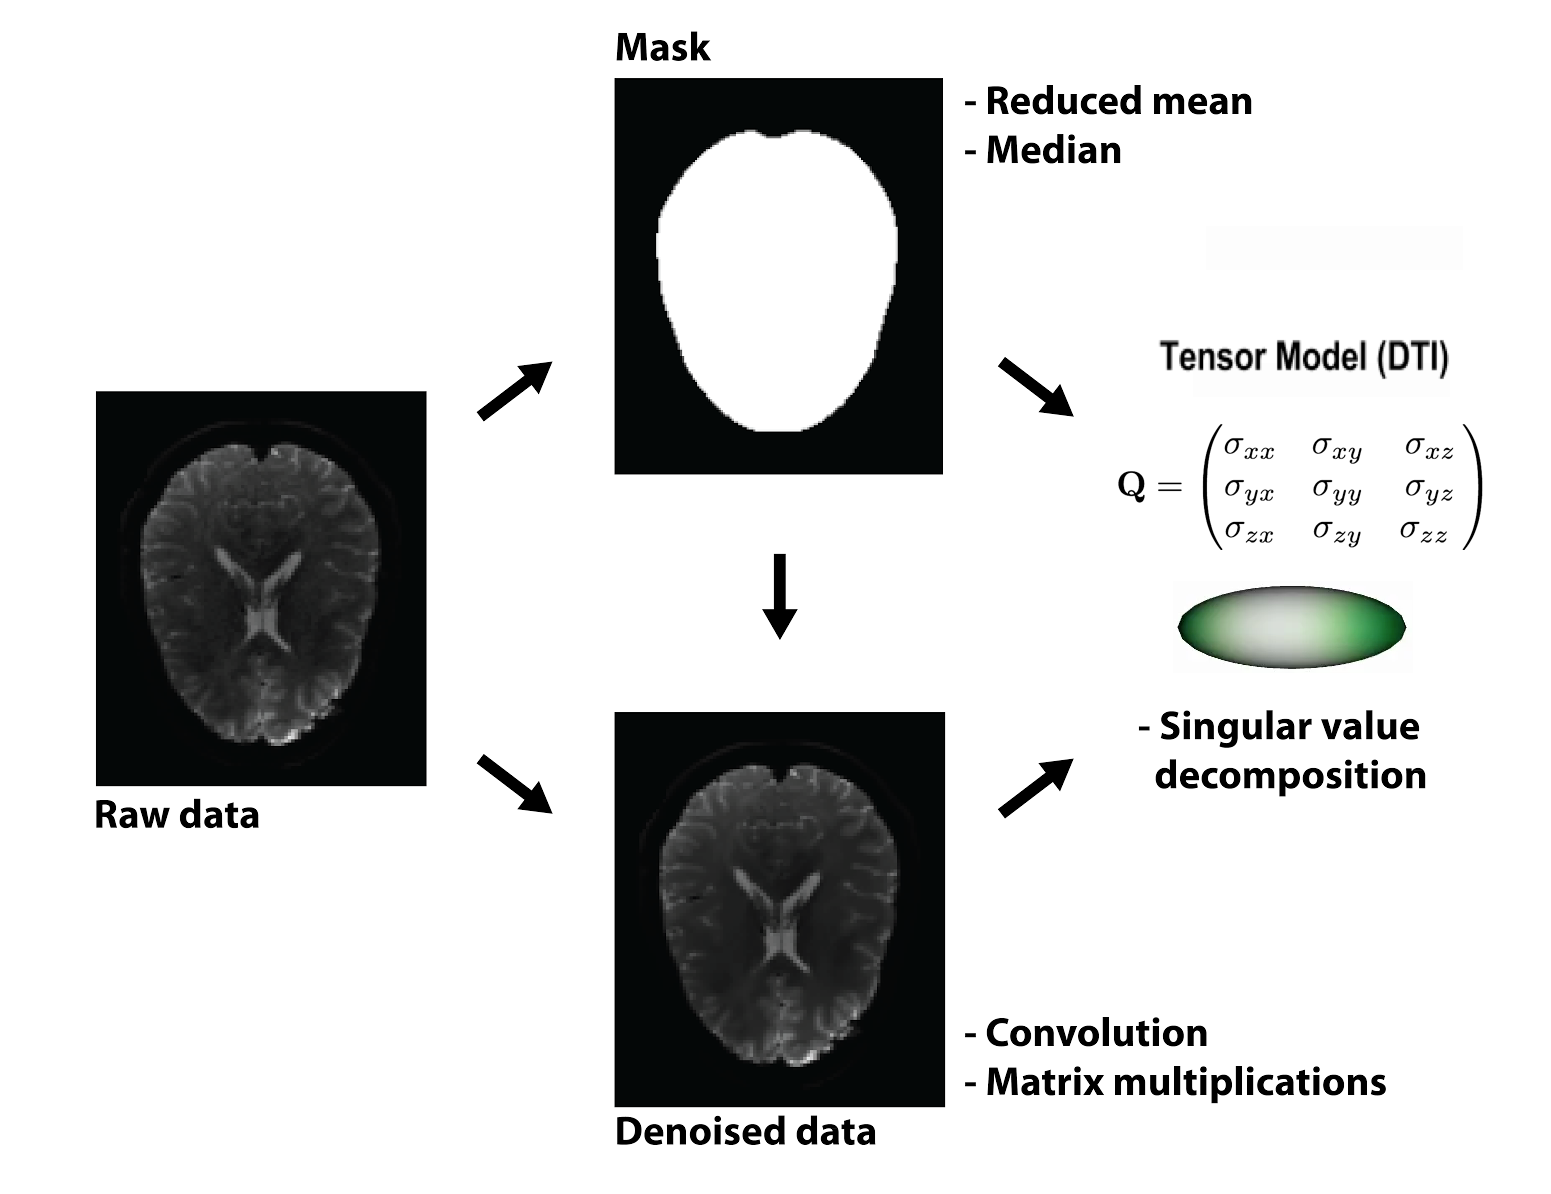
\includegraphics[width=25cm]{pipeline.png}

\begin{minipage}[b]{0.75\linewidth}
  Data analysis was based on functions implemented in the open-source Dipy
  software (\texttt{http://dipy.org}).
\end{minipage}
\begin{minipage}[b]{0.25\linewidth}
  
\includegraphics[width=5cm]{dipy-logo.png}
\end{minipage}

\subsection*{Computational experiments}
We used AWS r3.2xlarge instance type, optimized for memory-intensive applications (lower price per GiB of RAM): each instance has 8 vCPU, 61 GiB Memory and 160 GB SSD storage.

\textbf{Pure Python}: The reference implementation was run on a single instance.

\textbf{Myria}:  Four compute nodes and one master node. Each compute node ran
four workers making for a total of sixteen workers. For this image processing
pipeline, Myria was setup with PostgreSQL as the per-node, local storage layer (default configuration).

\textbf{Spark}: Four compute nodes and one master node, Each compute node ran
eight workers; spark default is one worker per CPU, for a total of thirty-two
workers. We used spark-1.6.1-bin-hadoop1, in standalone mode with HDFS as the
storage layer. We also used thunder 0.6.0 (\texttt{http://thunder-project.org/})
to set up spark.

\textbf{Rasdaman}: Four compute nodes were used and the default configuration:
nine Rasdaman server processes on each node. We made reasonable effort to push
certain application operations into Rasdaman’s query engine.

%------------------------------------------------


%----------------------------------------------------------------------------%	RESULTS
%----------------------------------------------------------------------------
\section*{Results}

\begin{minipage}[b]{0.5\linewidth}
  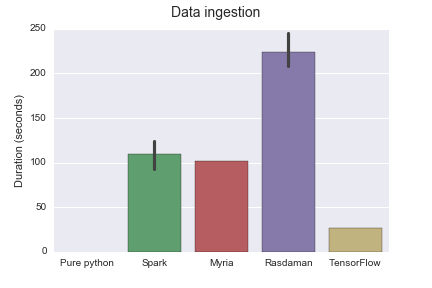
\includegraphics[width=17cm]{DataIngestion.png}
\end{minipage}
\begin{minipage}[b]{0.5\linewidth}
  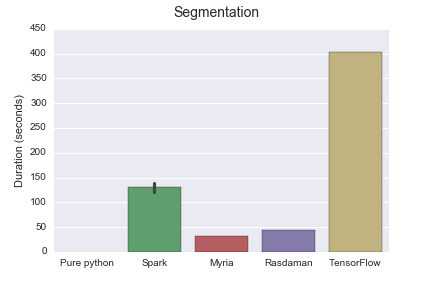
\includegraphics[width=17cm]{Segmentation.png}
\end{minipage}


\begin{minipage}[b]{0.5\linewidth}
  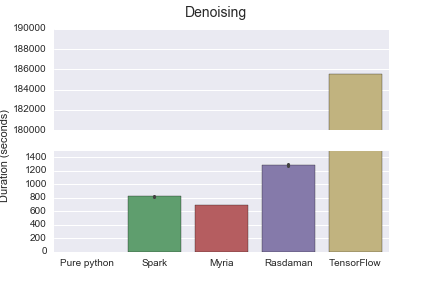
\includegraphics[width=17cm]{Denoising.png}
\end{minipage}
\begin{minipage}[b]{0.5\linewidth}
  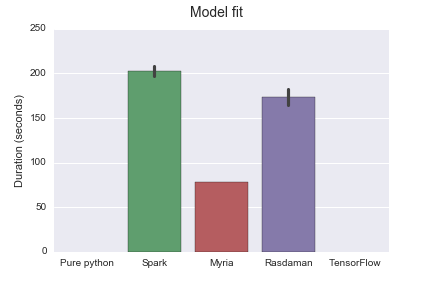
\includegraphics[width=17cm]{ModelFit.png}
\end{minipage}



\color{SaddleBrown} % SaddleBrown color for the conclusions to make them stand out

\section*{Conclusions}

\begin{itemize}

\item Myria performs faster than other systems for most tasks. This is probably due to reduced serialization cost, which other systems incur.

\item Rasdaman requires significant rewriting of algorithms to be used.

\item  Spark error handling can be cryptic, because it uses the JVM.

\item TensorFlow is still under heavy development, and might be much more performant in the future.

\end{itemize}

\color{DarkSlateGray} % Set the color back to DarkSlateGray for the rest of the content

%----------------------------------------------------------------------------%	Future directions
%----------------------------------------------------------------------------

\section*{Future directions}

Future developments include the development of user-defined aggregations in Myria.

Myria will also serve as the computational backend for web-based image processing pipelines we will provide as a service.

%---------------------------------------------------------------------------	REFERENCES
%----------------------------------------------------------------------------

\nocite{*} % Print all references regardless of whether they were cited in the poster or not
\bibliographystyle{plain} % Plain referencing style
\small \bibliography{poster} % Use the example bibliography file sample.bib

%----------------------------------------------------------------------------%	ACKNOWLEDGEMENTS
%----------------------------------------------------------------------------
\section*{Acknowledgements}

This research was supported through a grant from the Gordon \& Betty Moore
Foundation and the Alfred P. Sloan Foundation to the University of Washington
eScience Institute and through grants from the National Science Foundation


\includegraphics[height=2.5cm]{eSciencelogo.png}

\includegraphics[height=2.5cm]{SloanLogo.png}

\includegraphics[height=2.5cm]{MooreFdn.png}

\includegraphics[height=2.5cm]{NSFLogo}
%----------------------------------------------------------------------------

\end{multicols}
\end{document}
